\section{Methodology}
Initially we do a collection of bugs from Pyodide repo. We then go ahead to analyse these bugs and try to compare them to the bugs proosed by Romano et al. \cite{bugsinwasm}. 

\subsection{Bugs Collection}
Our first goal is data collection. We follow the methods proposed followed by \cite{bugsinwasm} and use Github Search API\cite{githubsearchapi} and Github REST API\cite{githubrestapi} to collect all issues and pull requests. The project has a total of 880 Closed and 277 Open issues at the time of collection. For our use case, we filter out all the issues with label bug. This brings the total issues down tp 149 (closed) + 43 (open). We go through a detailed analysis of each issue and seggregate them based on the categories as shown in table \ref{tab:categories_bugs}. For the scope of the research course, we look at only the closed issues and filter out all duplicate bugs, won't-fix bugs and any bugs in the build time of pyodide. We majorly look at issues that are posed which are more focused with respect to pyodide as a framework itself or one of it's dependency CPython, emscripten or WebAssembly amongst others\footnote{The complete list of bugs is avaialble on sheets \url{https://stagbin.tk/pyodide_issues}}.

\begin{table}[]
    \begin{tabular}{|l|l|}
        \hline
        \textbf{Category}               & \textbf{Number of Unique Issues}  \\ \hline
        Asyncify Synchronous Code       &           1                       \\ \hline
        Incompatible Data Type          &           3                       \\ \hline
        Memory Model Differences        &           7                       \\ \hline
        Other Infrastructure Bug        &           12                      \\ \hline
        Emulating Native Environment    &           1                       \\ \hline
        Supporting Web API's            &           1                       \\ \hline
        Pyodide Specific                &           21                      \\ \hline
    \end{tabular}
\caption{Categories of issues taken from \cite{bugsinwasm}}
\label{tab:categories_bugs}
\end{table}

\subsection{Analysis}
From figure \ref{fig:bug_analysis}, Pyodide specific bugs are the highest with 21 of the bugs belonging to the category, With other Infrastructure bugs being the immediate next. We briefly describe the basis on which we have categorized the bugs.
\subsection*{Pyodide Specific}
All the bugs that have occured purely due to the issue with coding styles, typos, or any other issue that is specific to pyodide. These bugs are mostly related to the core of the project and are not related to any of the dependencies. These also include the bugs that were introduced as a side effect of some other bug fix.
\subsection*{Other Infrastructure Bug}
These bugs are related to the dependencies of pyodide. These include bugs related to CPython, emscripten, WebAssembly, Asyncify, etc. These bugs are mostly related to the way the dependencies are used in pyodide. These could be further divided based on a deeper study of all issues into other relavant categories. But at this time we broadly separate all external dependent bugs into this category.
\subsection*{Memory Model Differences}
These are bugs which look at differences in the data types or the way storage is allocated to variables. For example transferring byte objects between pyodide and javascript\footnote{This issue can be found in $\#$749 in pyodide issues\cite{pyodide-issues}}. These bugs are mostly related to the way the data is stored in the memory and how it is accessed.
\subsection*{Incompatible Data Type}
These include issues that arise due to incompatibility of data types when compiling from one language to another. 
\subsection*{Supporting Web API's}
These are bugs which look at the support for web API's. Web Api's are the set of functions that are available in the browser. These are mostly related to the way the browser interacts with the code. For example, the issue of \texttt{Promise} object not being available in Pyodide.
\subsection*{Emulating Native Environment}
These are bugs that depend on native environment such as POSIX threads or POSIX signals. 
\subsection*{Asyncify Synchronous Code}
These are bugs that arise due to the use of synchronous code in the browser. 

\begin{figure}[h]
    \centering
    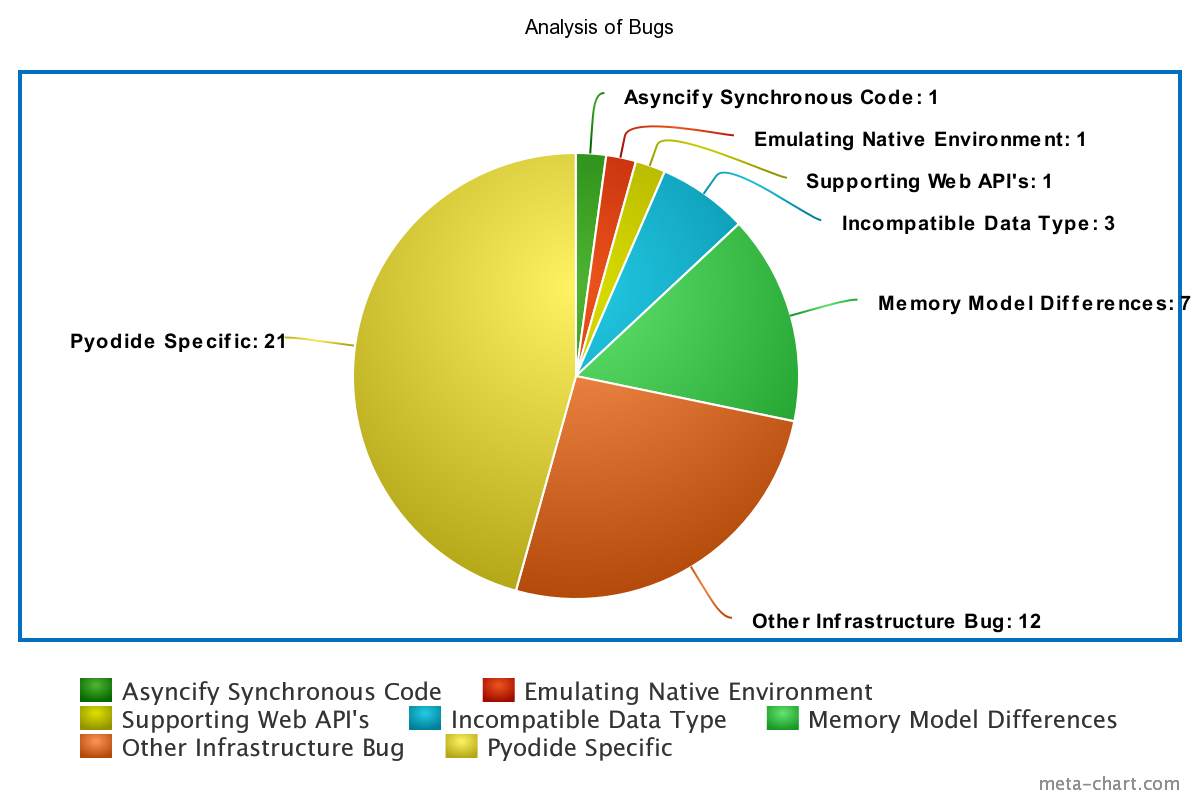
\includegraphics[width=0.8\linewidth]{images/meta-chart.png}
    \caption{Analysis of bugs}
    \label{fig:bug_analysis}
\end{figure}

\subsection{Impact of Bugs}
The impact of bugs in a bigger scope varies from project to project. For instance a bug that exists when installing scipy\footnote{https://github.com/pyodide/pyodide/pull/2348} in pyodide would be more relavant to a project focused towards Machine Learning. But for our use case with virtual labs, we are looking at the bugs that interfere with the requirements of Client Side Virtual Labs implementation. \\
From the study, we see majority of the bugs are geared towards issues specific to pyodide, installing libraries and to memory management, most of which do not directly impact the implementation of virtual labs. But there are a few bugs that are more relavant to our use case. To be specific we look at a major bugs we have identified. \\

\subsection*{Interrupting the execution of code}
Due to single threaded nature of javascript and the lack of signal handling, it is not possible to interrupt the execution of code. This is a major issue when it comes to implementing python virtual labs. For instance, in a virtual lab, the user is expected to be able to interrupt the execution of code at any point of time or to automatically stop the execution in case of an infinite loop. Pyodide suggests a solution with use of web workers\footnote{https://pyodide.org/en/stable/usage/webworker.html}. But this depends on Browsers having support for SharedArrayBuffer\footnote{https://developer.mozilla.org/en-US/docs/Web/JavaScript/Reference/Global\_Objects/SharedArrayBuffer}. This is not supported by all browsers and is still in experimental phase. To enable this, the server hosting the virtual lab needs to have the correct headers set. \\

